\documentclass[conference]{IEEEtran}
\IEEEoverridecommandlockouts
% The preceding line is only needed to identify funding in the first footnote. If that is unneeded, please comment it out.
\usepackage{cite}
\usepackage{amsmath,amssymb,amsfonts}
\usepackage{algorithmic}
\usepackage{graphicx}
\usepackage{textcomp}
\usepackage{xcolor}
\def\BibTeX{{\rm B\kern-.05em{\sc i\kern-.025em b}\kern-.08em
    T\kern-.1667em\lower.7ex\hbox{E}\kern-.125emX}}
\begin{document}

\title{Formal Verification of Integer Multiplier Circuits\\}

\author{
\IEEEauthorblockN{Jonathan Wang}
\IEEEauthorblockA{\textit{Price College of Engineering} \\
\textit{University of Utah}\\
Salt Lake City, Utah \\
u1306458@utah.edu}
\and
\IEEEauthorblockN{Henry Silverman}
\IEEEauthorblockA{\textit{Price College of Engineering} \\
\textit{University of Utah}\\
Salt Lake City, Utah \\
henry.silverman@utah.edu}
\and
\IEEEauthorblockN{Garrett Slack}
\IEEEauthorblockA{\textit{Price College of Engineering} \\
\textit{University of Utah}\\
Salt Lake City, Utah \\
u1315263@utah.edu}
\and
\IEEEauthorblockN{Dmitry Panin}
\IEEEauthorblockA{\textit{Price College of Engineering} \\
\textit{University of Utah}\\
Salt Lake City, Utah \\
dmitry.panin@utah.edu}
}

\maketitle

\begin{abstract}
This paper employs advanced mathematical techniques, specifically polynomials, and ideals, 
to rigorously verify the correctness of an integer multiplier circuit. By leveraging algebraic methods, 
this approach will provide a deeper understanding of the circuit's behavior and enable a more robust 
verification process. 
\end{abstract}

\begin{IEEEkeywords}
polynomials, ideals, multiplier circuit
\end{IEEEkeywords}

\section{Introduction}
The paper presents the testing and verification of a 2-bit, 3-bit, 16-bit, and 32-bit integer multiplier circuit. We manually 
designed the 2-bit and 3 bit multiplier from scratch and derived a polynomial spec. We generated the larger circuits utilizing 
the ABC synthesis tool.

\section{Approach}
Our approach to generate the 2-bit and 3-bit multiplier is simple for circuit generation,. We added on to the 2-bit multiplier 
provided by Dr. Kalla using the GEdit text editor. Then ran on command line in VMA RedHat Linux. For the larger 16-bit and 32-bit 
circuits, we generated the circuits using the ABC synthesis tool shown in Fig. 1. 
\begin{figure}[ht]
    \centering
    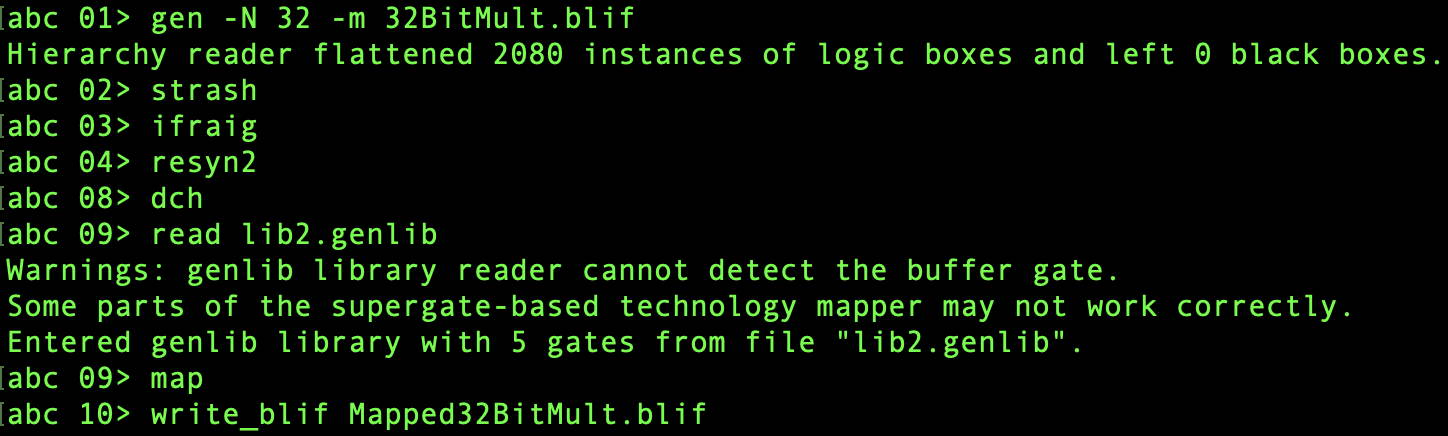
\includegraphics[scale = 0.34]{32bit_abc.png}
    \caption{Steps to generate a 32-bit circuit in ABC.}
    \label{fig}
\end{figure}

\section{Algorithms and Techniques}
Before you begin to format your paper, first write and save the content as a 
separate text file. Complete all content and organizational editing before 
formatting. Please note sections  below for more information on 
proofreading, spelling and grammar.

\section{Software implementations}
Before you begin to format your paper, first write and save the content as a 
separate text file. Complete all content and organizational editing before 
formatting. Please note sections  below for more information on 
proofreading, spelling and grammar.

\section{Concepts learned}
Before you begin to format your paper, first write and save the content as a 
separate text file. Complete all content and organizational editing before 
formatting. Please note sections  below for more information on 
proofreading, spelling and grammar.

\section{Labour Division}
Jonathan: a lot \\
Henry: a lot \\
Garrett: a lot \\
Dmitri: a lot

\begin{thebibliography}{00}
\bibitem{b1} D. Ritirc, A. Biere and M. Kauers, "Column-wise verification of multipliers using computer algebra," 2017 Formal Methods in Computer Aided Design (FMCAD), Vienna, Austria, 2017, pp. 23-30, doi: 10.23919/FMCAD.2017.8102237.
\bibitem{b2} T. Pruss, P. Kalla and F. Enescu, "Efficient Symbolic Computation for Word-Level Abstraction From Combinational Circuits for Verification Over Finite Fields," in IEEE Transactions on Computer-Aided Design of Integrated Circuits and Systems, vol. 35, no. 7, pp. 1206-1218, July 2016, doi: 10.1109/TCAD.2015.2501301.
\end{thebibliography}
\vspace{12pt}

\end{document}
